\subsection{Image\-Sum  Class Reference}
\label{class_imagesum}\index{ImageSum@{Image\-Sum}}
A class that handles coadding. Shift and coadd is handled by. 


{\tt \#include $<$imagesum.h$>$}

Inheritance diagram for Image\-Sum::\begin{figure}[H]
\begin{center}
\leavevmode
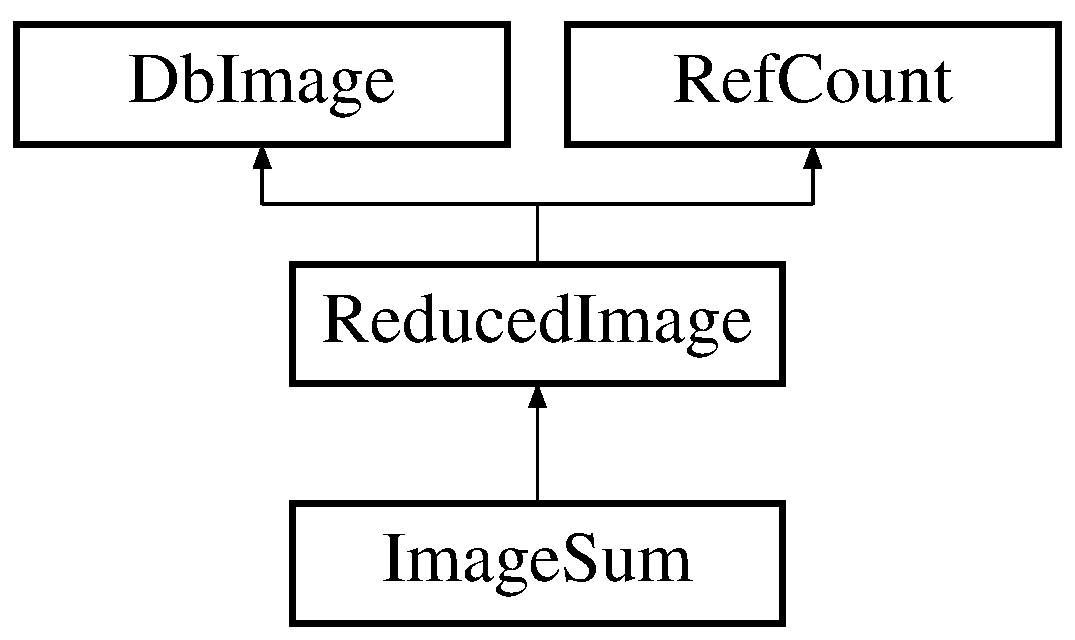
\includegraphics[height=3cm]{class_imagesum}
\end{center}
\end{figure}
\subsubsection*{Public Types}
\begin{CompactItemize}
\item 
\index{ComponentIterator@{ComponentIterator}!ImageSum@{Image\-Sum}}\index{ImageSum@{ImageSum}!ComponentIterator@{Component\-Iterator}}
typedef vector$<${\bf Component}$>$::iterator {\bf Component\-Iterator}\label{class_imagesum_s0}

\item 
\index{ComponentCIterator@{ComponentCIterator}!ImageSum@{Image\-Sum}}\index{ImageSum@{ImageSum}!ComponentCIterator@{Component\-CIterator}}
typedef vector$<${\bf Component}$>$::const\_\-iterator {\bf Component\-CIterator}\label{class_imagesum_s1}

\end{CompactItemize}
\subsubsection*{Public Methods}
\begin{CompactItemize}
\item 
\index{ImageSum@{ImageSum}!ImageSum@{Image\-Sum}}\index{ImageSum@{ImageSum}!ImageSum@{Image\-Sum}}
{\bf Image\-Sum} (const string \&Name, Reduced\-Image\-List \&Images, const {\bf Reduced\-Image} $\ast$Photom\-Reference=NULL, const Weighting\-Method AWMethod=WUn\-Set, const Stacking\-Method ASMethod=SUn\-Set)\label{class_imagesum_a0}

\item 
\index{ImageSum@{ImageSum}!ImageSum@{Image\-Sum}}\index{ImageSum@{ImageSum}!ImageSum@{Image\-Sum}}
{\bf Image\-Sum} (const string \&Name)\label{class_imagesum_a1}

\item 
\index{ImageSum@{ImageSum}!ImageSum@{Image\-Sum}}\index{ImageSum@{ImageSum}!ImageSum@{Image\-Sum}}
{\bf Image\-Sum} ()\label{class_imagesum_a2}

\item 
\index{Components@{Components}!ImageSum@{Image\-Sum}}\index{ImageSum@{ImageSum}!Components@{Components}}
Reduced\-Image\-List {\bf Components} () const\label{class_imagesum_a3}

\item 
\index{MakeFits@{MakeFits}!ImageSum@{Image\-Sum}}\index{ImageSum@{ImageSum}!MakeFits@{Make\-Fits}}
bool {\bf Make\-Fits} ()\label{class_imagesum_a4}

\begin{CompactList}\small\item\em produce fits image.\item\end{CompactList}\item 
\index{MakeCatalog@{MakeCatalog}!ImageSum@{Image\-Sum}}\index{ImageSum@{ImageSum}!MakeCatalog@{Make\-Catalog}}
bool {\bf Make\-Catalog} ()\label{class_imagesum_a5}

\begin{CompactList}\small\item\em Produce the Saturated stars pixels mask, subtract the image background, detect with the SExtractor computed sigma. search the cosmics, and update catalog and weight for cosmics. No free coffee.\item\end{CompactList}\item 
\index{MakeDead@{MakeDead}!ImageSum@{Image\-Sum}}\index{ImageSum@{ImageSum}!MakeDead@{Make\-Dead}}
bool {\bf Make\-Dead} ()\label{class_imagesum_a6}

\begin{CompactList}\small\item\em produce dead image.\item\end{CompactList}\item 
\index{MakeSatur@{MakeSatur}!ImageSum@{Image\-Sum}}\index{ImageSum@{ImageSum}!MakeSatur@{Make\-Satur}}
bool {\bf Make\-Satur} ()\label{class_imagesum_a7}

\begin{CompactList}\small\item\em produce satur image.\item\end{CompactList}\item 
\index{MakeWeight@{MakeWeight}!ImageSum@{Image\-Sum}}\index{ImageSum@{ImageSum}!MakeWeight@{Make\-Weight}}
bool {\bf Make\-Weight} ()\label{class_imagesum_a8}

\item 
\index{Create@{Create}!ImageSum@{Image\-Sum}}\index{ImageSum@{ImageSum}!Create@{Create}}
bool {\bf Create} (const string \&Where)\label{class_imagesum_a9}

\begin{CompactList}\small\item\em To create the directories where the fits images, catalogues will be put: ex: $\sim$/Fake\-Db/test: {\bf Db\-Image} {\rm (p.\,\pageref{class_dbimage})} dbim(\char`\"{}test\char`\"{}); dbim.Create(\char`\"{}$\sim$/Fake\-Db/\char`\"{});.\item\end{CompactList}\item 
\index{Clone@{Clone}!ImageSum@{Image\-Sum}}\index{ImageSum@{ImageSum}!Clone@{Clone}}
{\bf Reduced\-Image}$\ast$ {\bf Clone} () const\label{class_imagesum_a10}

\item 
\index{dump@{dump}!ImageSum@{Image\-Sum}}\index{ImageSum@{ImageSum}!dump@{dump}}
void {\bf dump} (ostream \&s=cout) const\label{class_imagesum_a11}

\begin{CompactList}\small\item\em dumps basic info.\item\end{CompactList}\item 
\index{ClassDef@{ClassDef}!ImageSum@{Image\-Sum}}\index{ImageSum@{ImageSum}!ClassDef@{Class\-Def}}
{\bf Class\-Def} (Image\-Sum, 1)\label{class_imagesum_a12}

\item 
\index{~ImageSum@{$\sim$ImageSum}!ImageSum@{Image\-Sum}}\index{ImageSum@{ImageSum}!~ImageSum@{$\sim$Image\-Sum}}
{\bf $\sim$Image\-Sum} ()\label{class_imagesum_a13}

\end{CompactItemize}


\subsubsection{Detailed Description}
A class that handles coadding. Shift and coadd is handled by.

Shift is performed using the {\bf Transformed\-Image} {\rm (p.\,\pageref{class_transformedimage})} class. Addition is performed using Image\-Sum. Depending on the numner of images involved, we perform either an actual sum, or a \char`\"{}clipped mean\char`\"{}. 



The documentation for this class was generated from the following file:\begin{CompactItemize}
\item 
{\bf imagesum.h}\end{CompactItemize}
